% --------------------------------------------------------------------------------

\begin{exercise}

Betrachten Sie die \textit{Helmholtz-Gleichung}

\begin{align*}
  (\Delta + k^2) u = f ~\text{in}~ \R^3
\end{align*}

mit der Wellenzahl $k > 0$, der Wellenquelle $f \in \mathcal{D}(\R^3)$ und dem Wellenfeld $u: \R^3 \to \C$.

\begin{enumerate}[label = (\roman*)]

  \item Berechnen Sie eine radialsymmetrische Funktion $G(x, \xi) = g(|x - \xi|)$,
  für die $(\Delta_x + k^2)G = \delta_\xi$ gilt, und die der \textit{sommerfeldschen
  Ausstrahlungsbedingung}

  \begin{align*}
    \lim_{r \to \infty} r \pbraces{\pderivative{r} - i k} g(r) = 0
  \end{align*}

  genügt.

  \textit{Anmerkung:}
  Diese Bedingung stellt eine Randbedingung (im Unendlichen) dar, weshalb man $G$ auch eine greensche Funktion nennt.

  \item Stellen Sie die/eine Lösung $u$ der Helmholtz-Gleichung mit Hilfe von $G(x, \xi)$ dar.
  Zeigen Sie, dass für eine radialsymmetrische Funktion $f$ diese Lösung auch radialsymmetrisch ist.

  \item Konstruieren Sie aus $G$ zwei weitere Funktionen $G_{\mathrm{Dir}}$ und $G_{\mathrm{Neu}}$, welche greensche Funktionen auf $\Omega := \R^2 \times \R_+$ sind und auf $\partial\Omega$ homogene Dirichlet- bzw. homogene Neumann-Randbedingunen erfüllen.

\end{enumerate}

\end{exercise}

% --------------------------------------------------------------------------------

\begin{solution}
\begin{enumerate}[label = (\roman*)]
\item Da unser Ableitungsoperator nur konstante Koeffizienten hat suchen wir eine Lösung mit Pol in $0$ und verschieben diese dann nach Satz $3.21$, den wir anwenden können da unser Differentialoperator ja konstante Koeffizienten hat, um eine Polstelle in $\xi$ zu erhalten.
Unsere Funktion $g$ soll nun radialsymmetrisch sein mit Radius $r = |x| = \sqrt{x_1^2 + x_2^2 +x_3^2}$.Wir berechnen zuerst für $i \in \{1,2,3\}$

\begin{align*}
  \frac{\partial r}{\partial x_i}
  =
  \frac{x_i}{\sqrt{x_1^2 + x_2^2 + x_3^2}}
  =
  \frac{x_i}{r}
\end{align*}

Dann gilt

\begin{align*}
  \frac{\partial G}{\partial x_i}
  =
  g^\prime (r) \frac{\partial r}{\partial x_i}
  =
  g^\prime (r) \frac{x_i}{r}
\end{align*}

Ferner ist

\begin{align*}
  \frac{\partial^2 G}{\partial x_i^2}
  =
  g^\primeprime(r) \frac{x_i^2}{r^2}
    + g^\prime(r) \frac{1}{r}
    - g^\prime(r) \frac{x_i}{r}\frac{x_i}{r^2}
\end{align*}

Also erhalten wir insgesamt

\begin{align*}
  (\Delta_x +k^2) G
  =
  \sum_{i=1}^3 \frac{\partial^2 G}{\partial x_i^2} + k^2 G
  =
  g^\primeprime(r) \sum_{i=1}^3 \frac{x_i^2}{r^2}
    + g^\prime(r) \frac{3}{r}
    - g^\prime(r) \sum_{i=1}^3 \frac{x_i^2}{r^3}
    + k^2 g(r)
  =
  g^\primeprime(r) + \frac{2}{r} g^\prime(r) + k^2g(r)
\end{align*}

Also wird $(\Delta_x +k^2) G = 0$ zu einer gewöhnlichen Differentialgleichung für $g$ die für $r>0$ zu lösen ist.

\begin{align*}
  0 = g^\primeprime(r) + \frac{2}{r} g^\prime(r) + k^2g(r)
\end{align*}

Durch Multiplikation mit $r$ und unter der Verwendung der Produktregel bekommen wir

\begin{align*}
  \frac{\partial^2}{\partial r^2}(rg) + k^2(rg) = 0
\end{align*}

Lösungen dieser Differentialgleichung sind gegeben durch $g = C \frac{1}{r}e^{\pm ikr}, C \in \C$. Um der sommerfeldschen Ausstrahlungsbedingung zu genügen
wählen wir $g = C \frac{1}{r}e^{ikr}$ mit der noch unbestimmten Konstante $C$ und rechnen nach

\begin{multline*}
  \lim_{r \to \infty} r \pbraces{\pderivative{r} - i k} g(r)
  =
  \lim_{r \to \infty} r \pbraces{C \frac{ik e^{ikr}r - e^{ikr}}{r^2} - ikC e^{ikr} \frac{1}{r}} \\
  =
  \lim_{r \to \infty} r \pbraces{\frac{1}{r^2} e^{ikr}(ikr - 1) - ikC e^{ikr} \frac{1}{r}}
  =
  \lim_{r \to \infty} \frac{1}{r} e^{ikr}ikr C - \frac{1}{r}e^{ikr}C - e^{ikr}ik C
  =
  0
\end{multline*}

Um zu zeigen, dass die Funktion $G(x, \xi) = g(|x - \xi|)$ auch Fundamentallösung ist sei $\phi \in \mathcal{D}(\R^3)$ beliebig, $\Omega_\varepsilon = \R^3 \setminus B_\varepsilon(0)$, dann ist (mit PI nach Gauss)

\begin{align*}
  \langle (\Delta_x + k^2)G(\cdot, 0), \phi \rangle
  &=
  \langle G(\cdot, 0), (\Delta_x + k^2) \phi \rangle
  =
  \Int[\Omega_\varepsilon]{G(x, 0) (\Delta + k^2) \phi(x)}{x} \\
  &=
  \Int[\Omega_\varepsilon]{G(x, 0) \Delta \phi(x)}{x} + \Int[\Omega_\varepsilon]{G(x, 0)k^2 \phi(x)}{x} \\
  &=
  -\Int[\Omega_\varepsilon]{\nabla G(x, 0) \cdot \nabla \phi(x)}{x}
    + \Int[\Omega_\varepsilon]{G(x, 0)k^2 \phi(x)}{x}
    + \Int[\partial \Omega_\varepsilon]{G(x,0) \nabla \phi \cdot \nu}{s} \\
  &=
  \underbrace{\Int[\Omega_\varepsilon]{(\Delta_x + k^2)G(x, 0) \phi(x)}{x}}_{=0}
    + \Int[\partial \Omega_\varepsilon]{G(x,0) \nabla \phi \cdot \nu}{s}
    - \Int[\partial \Omega_\varepsilon]{\phi \nabla G(x,0) \cdot \nu}{s} \\
\end{align*}

Die beiden Randintegrale schauen wir uns für $\varepsilon \rightarrow 0$ noch einmal genauer an.

\begin{align*}
  \pbraces{\Int[\partial \Omega_\varepsilon]{G(x,0) \nabla \phi \cdot \nu}{s}}
  \leq
  \underbrace{|g(\varepsilon)|}_{\frac{C}{\varepsilon}} \underbrace{\text{meas}(\partial \Omega_\varepsilon)}_{\varepsilon^2 S_3} \max_{x \in \R^3}|\nabla \phi(x)|
  \stackrel{\varepsilon \to 0}{\longrightarrow}
  0
\end{align*}

Beim zweiten verwenden wir $\nu(x) = - r$, wenden den MWS der Integralrechnung an und wählen $C = -\frac{1}{S_3}$

\begin{align*}
  - \Int[\partial \Omega_\varepsilon]{\phi \nabla g(|x|) \cdot \nu}{s}
  &\stackrel{\text{MWS}}{=}
  \phi(x_\varepsilon) \frac{\partial g}{\partial r}(\varepsilon) \Int[\partial \Omega_\varepsilon]{1}{s} \\
  =
  \phi(x_\varepsilon) C \frac{ik e^{ik\varepsilon}\varepsilon - e^{ik\varepsilon}}{\varepsilon^2} \varepsilon^2 S_3
  &=
  -\phi(x_\varepsilon) \underbrace{(ik e^{ik\varepsilon}\varepsilon - e^{ik\varepsilon})}_{\stackrel{\varepsilon \to 0}{\longrightarrow} -1}
  \stackrel{\varepsilon \to 0}{\longrightarrow}
  \phi(0)
\end{align*}
Also insgesamt

\begin{align*}
  \langle (\Delta_x + k^2)G(\cdot, 0), \phi \rangle
  =
  \langle \delta, \phi \rangle
\end{align*}

\item Um eine Lösung mit $G(x,\xi)$ darzustellen verwenden wir wieder Satz $3.21$.

\begin{figure}[h!]
  \centering
  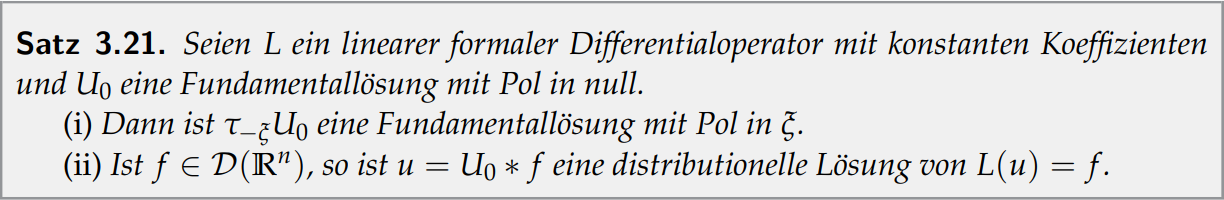
\includegraphics
  [width = 0.75 \textwidth]
  {Satz 3-21.png}
\end{figure}

Dieser besagt, dass $G(x,0) \ast f$ eine distributionelle Lösung von $L(u) = f$ ist.
Mit den Rechenregeln für Distributionen gilt $\Forall \phi \in \mathcal{D}(\Omega):$

\begin{multline*}
  \langle g \ast f, \phi \rangle
  =
  \langle g, \phi \ast Rf \rangle
  =
  \Int[\R^3]{g(|y|)(\phi \ast Rf)(y)}{y}
  =
  \Int[\R^3]
  {
    \Int[\R^3]
    {
      g(|y|)
      f(x - y)
      \phi(x)
    }{x}
  }{y} \\
  =
  \Int[\R^3]
  {
    \Int[\R^3]
    {
      g(|y|)
      f(x - y)
    }{y}
    \phi(x)
  }{x}
  =
  \abraces
  {
    \Int[\R^3]
    {
      g(|y|)
      f(x - y)
    }{y},
    \phi
  }
\end{multline*}

wobei $(Rf)(x) = f(-x)$ und die zweite Gleichheit wegen $g \in L^1_{\mathrm{loc}}(\R^3)$ gilt. Daher ist

\begin{align*}
  (G(x,0) \ast f)(x)
  =
  \Int[\R^3]{g(|y|) f(x-y)}{y}
\end{align*}

Weil $f$ eine Testfunktion ist, ist die Faltung $G \ast f \in C^{\infty}(\R^3)$ und damit auch eine klassische Lösung.

Um einzusehen, dass die Lösung für rotationssymmetrisches $f$ auch rotationssymmetrisch ist seien $x_1, x_2 \in \R^3$ mit
$|x_1| = |x_2|$ und $R$ die Rotationsabbildung, die $x_2$ auf $x_1$ abbildet.
Unter Ausnutzung der Rotationssymmetrie von $g$ und $f$ erhalten wir

\begin{align*}
  (g \ast f)(x_1)
  =
  \Int[\R^3]{g(|x_1|) f(|x_1 - y|)}{y}
  = \Int[\R^3]{g(|R(x_1)|) f(|R(x_1 - y)|)}{y} \\
  =
  \Int[\R^3]{g(|x_2|) f(|x_2 - Ry|) }{y}
  \stackrel{TRAFO}{=} \Int[\R^3]{g(|x_2|) f(|x_2 - u|) \underbrace{|\det(R^{-1})|}_{=1}}{u} =
  (g \ast f)(x_2)
\end{align*}

\item Wir schreiben noch einmal genau auf, was $G_{\mathrm{Dir}}$ und $G_{\mathrm{Neu}}$ erfüllen sollen:

\begin{align*}
  \Delta G_\mathrm{Dir}(\cdot, \xi) = \delta_\xi ~\text{in}~ \Omega,&
  \quad
  G_\mathrm{Dir}(\cdot, \xi) = 0 ~\text{auf}~ \partial \Omega \\
  \Delta G_\mathrm{Neu}(\cdot, \xi) = \delta_\xi ~\text{in}~ \Omega,&
  \quad
  \frac{\partial G_\mathrm{Neu}}{\partial \nu}(\cdot, \xi) = 0 ~\text{auf}~ \partial \Omega
\end{align*}

Um die Dirichlet-Randbedingung zu erfüllen Spiegeln wir in der $(x,y)-$Ebene und erhalten so mit $x = (x_1,x_2,x_3), \xi = (\xi_1, \xi_2, \xi_3)$

\begin{align*}
  G_\mathrm{Dir}(x,\xi) = G(x,(\xi_1, \xi_2, \xi_3)) - G(x,(\xi_1,\xi_2, -\xi_3))
\end{align*}

Diese Funktion hat in $\Omega$ nur den Pol $(\xi_1, \xi_2, \xi_3)$ und erfüllt somit die erste Bedingung. Die Randbedingung rechnen wir nach:
\begin{align*}
  G((x_1,x_2,0),(\xi_1, \xi_2, \xi_3)) - G((x_1,x_2,0),(\xi_1,\xi_2, -\xi_3))
  = \\
  -\frac{1}{S_3}\left(\frac{e^{ik\sqrt{(x_1 - \xi_1)^2 + (x_2 - \xi_2)^2 + \xi_3^2 }}}{\sqrt{(x_1 - \xi_1)^2 + (x_2 - \xi_2)^2 + \xi_3^2 }}
    -\frac{e^{ik\sqrt{(x_1 - \xi_1)^2 + (x_2 - \xi_2)^2 + \xi_3^2 }}}{\sqrt{(x_1 - \xi_1)^2 + (x_2 - \xi_2)^2 + \xi_3^2 }}\right)
  =
  0
\end{align*}

Um die Neumann-Randbedingunen zu erfüllen, Spiegeln wir ebenfalls aber addieren die Funktionen

\begin{align*}
  G_\mathrm{Neu}(x,\xi) = G(x,(\xi_1, \xi_2, \xi_3)) + G(x,(\xi_1,\xi_2, -\xi_3))
\end{align*}

Auch diese hat in $\Omega$ nur einen Pol und die Randbedingung rechnen wir wieder nach, wobei der Normalenvektor durch $\nu = (0,0,-\xi_3)$ gegeben ist.

\begin{align*}
  S_3\frac{\partial G_\mathrm{Neu}}{\partial \nu}(x, \xi)
  =
  -S_3\frac{\partial G_\mathrm{Neu}}{\partial \xi_3}(x, \xi)
  =
  -S_3(\frac{\partial G}{\partial \xi_3}((x_1,x_2,0),(\xi_1, \xi_2, \xi_3)) + \frac{\partial G}{\partial \xi_3}((x_1,x_2,0),(\xi_1,\xi_2, -\xi_3))) \\
  =
  \dfrac{\left(-{\xi}_3\right)\mathrm{e}^{\mathrm{i}k\sqrt{\left(-{\xi}_3\right)^2+\left(x_2-{\xi}_2\right)^2+
  \left(x_1-{\xi}_1\right)^2}}}{\left(\left(-{\xi}_3\right)^2+\left(x_2-{\xi}_2\right)^2+
  \left(x_1-{\xi}_1\right)^2\right)^\frac{3}{2}}
  +
  \dfrac{\mathrm{i}k\left(-{\xi}_3\right)\mathrm{e}^{\mathrm{i}k
  \sqrt{\left(-{\xi}_3\right)^2+\left(x_2-{\xi}_2\right)^2+\left(x_1-{\xi}_1\right)^2}}}{\left(-{\xi}_3\right)^2+
  \left(x_2-{\xi}_2\right)^2+\left(x_1-{\xi}_1\right)^2} \\
  +
  \dfrac{\mathrm{i}k\xi_3\mathrm{e}^{\mathrm{i}k\sqrt{\xi_3^2+\left(x_2-{\xi}_2\right)^2+
  \left(x_1-{\xi}_1\right)^2}}}{\xi_3^2+\left(x_2-{\xi}_2\right)^2+\left(x_1-{\xi}_1\right)^2}
  +
  \dfrac{\xi_3\mathrm{e}^{\mathrm{i}k\sqrt{\xi_3^2+\left(x_2-{\xi}_2\right)^2+
  \left(x_1-{\xi}_1\right)^2}}}{\left(\xi_3^2+\left(x_2-{\xi}_2\right)^2+\left(x_1-{\xi}_1\right)^2\right)^\frac{3}{2}}
  =
  0
\end{align*}
\end{enumerate}
\end{solution}

% --------------------------------------------------------------------------------
